\documentclass[10pt]{beamer}

%% Based on the original theme by Matthias Vogelgesang

\usetheme[progressbar=frametitle]{metropolis}
\usepackage{appendixnumberbeamer}

\usepackage{booktabs}
\usepackage[scale=2]{ccicons}

\usepackage{pgfplots}
\usepgfplotslibrary{dateplot}

\usepackage{xspace}
\usepackage{xcolor}
\newcommand{\themename}{\textbf{\textsc{metropolis}}\xspace}

%%%%%%%%%%%%%%%%%%%%%%%%%%%%
%% UNCC Theme Adjustments %%
%%%%%%%%%%%%%%%%%%%%%%%%%%%%
\definecolor{CanvasBG}{HTML}{FAFAFA}

% From the official style guide
\definecolor{UnccGreen}{HTML}{00703C}
\definecolor{UnccGold}{HTML}{B3A369}
\definecolor{UnccLightGreen}{HTML}{C3D7A4}
\definecolor{UnccYellow}{HTML}{F0CB00}
\definecolor{UnccOrange}{HTML}{F3901D}
\definecolor{UnccLightYellow}{HTML}{FFF6DC}
\definecolor{UnccBlue}{HTML}{00728F}
\definecolor{UnccPink}{HTML}{DE3A6E}
\definecolor{White}{HTML}{FFFFFF}
\definecolor{LightGray}{HTML}{DDDDDD}

% Supporting Color Palette
\definecolor{WarmGray}{HTML}{696158}
\definecolor{StoneGray}{HTML}{717C7D}
\definecolor{DarkGreen}{HTML}{2C5234}
\definecolor{LightGreen}{HTML}{509E2F}
\definecolor{BrightGold}{HTML}{F0CB00}

% Screamers
\definecolor{Royal}{HTML}{72246C}
\definecolor{Ocean}{HTML}{006BA6}
\definecolor{Flash}{HTML}{B52555}
\definecolor{Citrus}{HTML}{FFB81C}
\definecolor{Spring}{HTML}{CEDC00}

% Serenity
\definecolor{Garden}{HTML}{B7CE95}
\definecolor{Sand}{HTML}{F0E991}
\definecolor{Bloom}{HTML}{F1E6B2}
\definecolor{Clay}{HTML}{B7B09C}
\definecolor{Cloud}{HTML}{BAC5B9}

% Set colors here
\setbeamercolor{frametitle}{bg=UnccGreen}
\setbeamercolor{progress bar}{bg=BrightGold, fg=UnccGreen}
\setbeamercolor{alerted text}{fg=Flash}

\setbeamercolor{block title}{bg=LightGreen, fg=White}
\setbeamercolor{block title example}{bg=Ocean, fg=White}
\setbeamercolor{block title alerted}{bg=Citrus, fg=White}
\setbeamercolor{block body}{bg=CanvasBG}
\setbeamersize{text margin left=5mm,text margin right=5mm} 

\metroset{titleformat=smallcaps, progressbar=foot, sectionpage=none}

\makeatletter
\setlength{\metropolis@progressinheadfoot@linewidth}{2pt}
\setlength{\metropolis@titleseparator@linewidth}{2pt}
\setlength{\metropolis@progressonsectionpage@linewidth}{2pt}
%%%%%%%%%%%%%%%%%%%%%%%%%%%%
%% UNCC Theme Adjustments %%
%%%%%%%%%%%%%%%%%%%%%%%%%%%%


\title{Abschlussvortrag}
\subtitle{Sensorbasierter Orientierungssinn\\mit künstlichen neuronalen Netzen\\und Entscheidungsbäumen}
\date{16.06.2021}
\author{Tom Dymel}
\institute{Masterarbeit\\Technische Universität Hamburg}

\begin{document}

\maketitle

\section{Einleitung}
\begin{frame}{Motivation und Ziele}
\begin{itemize}
    \item Motivation
    \begin{itemize}
        \item Orientierungssinn von Tieren und Menschen
        \item Mian untersuchte FFNN und simulierte Daten
        \item Entscheidungsbäume potentiell effizienter
    \end{itemize}
    \item Ziele
    \begin{itemize}
        \item Diskrete Standortbestimmung % Definiere an dieser Stelle diesen Begriff mündlich
        \item Nutzung von mehreren Sensoren
        \item Ausgewählte Features bewerten
    \end{itemize}
\end{itemize}
\end{frame}

% Unterteilen die Route in sich auschließende Teile
% Eine Sensorenbox nimmt zu jedem Zeitpunkt versch. Sensorwerte auf
% Diese werden zu Features verarbeitet
% Problem wird als Klassifizierungsproblem modelliert
\begin{frame}{Ansatz zur diskreten Standortbestimmung I}
    \begin{figure}
        \centering
        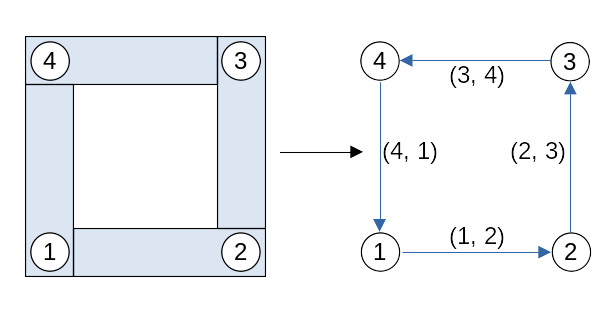
\includegraphics[width=\linewidth]{model/location_encoding.png}
    \end{figure}
\end{frame}

\begin{frame}{Ansatz zur diskreten Standortbestimmung II}
    \begin{figure}
        \centering
        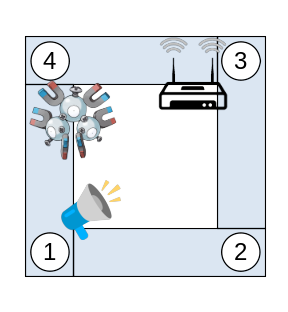
\includegraphics[width=0.6\linewidth]{model/grundlegender_ansatz_2.png}
    \end{figure}
\end{frame}

\begin{frame}{Sensoren}
\begin{minipage}{.5\textwidth}
    \begin{itemize}
        \item Accelerometer
        \item Gyroskop
        \item Licht
        \color{red}
        \item Magnetfeld
        \item Temperatur
        \item Geräusche
        \item WLAN-Zugangspunkte
    \end{itemize}
\end{minipage}%
\begin{minipage}{.5\textwidth}
    \centering
    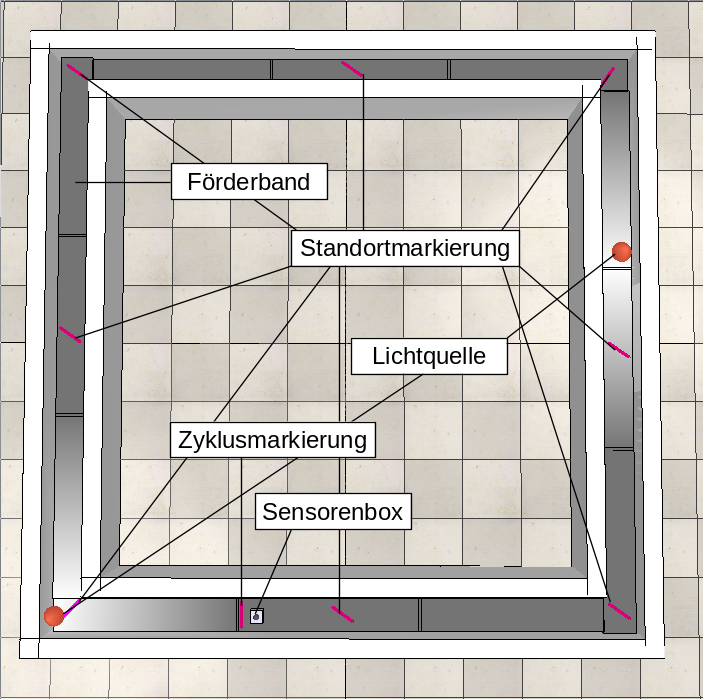
\includegraphics[width=\linewidth]{model/simple_square_labeled.png} 
\end{minipage}
\end{frame}

\section{Modell}
\begin{frame}{Modell}
    \begin{figure}
        \centering
        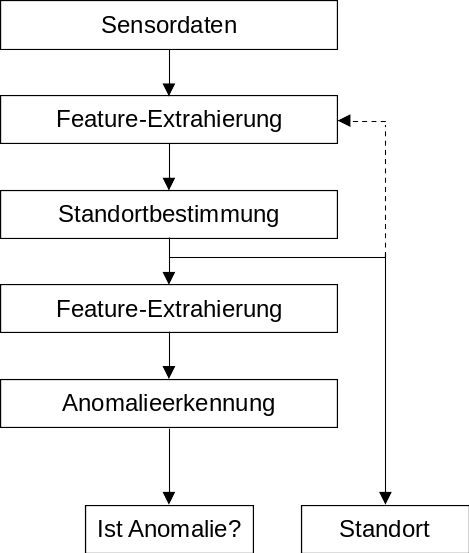
\includegraphics[width=0.55\linewidth]{model/model_vertical.png}
    \end{figure}
\end{frame}

\section{Standorterkennung}
% Gehe hier auf das Datenfenster ein
\begin{frame}{Extrahierte Features}
    \begin{table}
        \centering
        \begin{tabular}{ | l | c | c | c | c | c | }
            \hline
            Sensordaten & $\sigma$ & Min. & Max. & Ø & Wert \\\hline
            Accelerometer & X & X & X & X & X \\\hline
            Gyroskop & X & X & X & X & X \\\hline
            Ausrichtung zum Magnetfeld & X & X & X & X & X \\\hline
            Temperatur & X & X & X & X & X \\\hline
            Licht & X & X & X & X & X \\\hline
            Geräusch & X & X & X & X & X \\\hline
            WLAN-Zugangspunkte & - & - & - & - & X \\\hline
            Letzter Standort & - & - & - & - & X \\\hline
            Letzter unterschiedlicher Standort & - & - & - & - & X \\\hline
            Zeit & X & - & - & - & - \\\hline
        \end{tabular}
    \end{table}
\end{frame}

\begin{frame}{Training der ML-Modelle}
    \begin{figure}
        \centering
        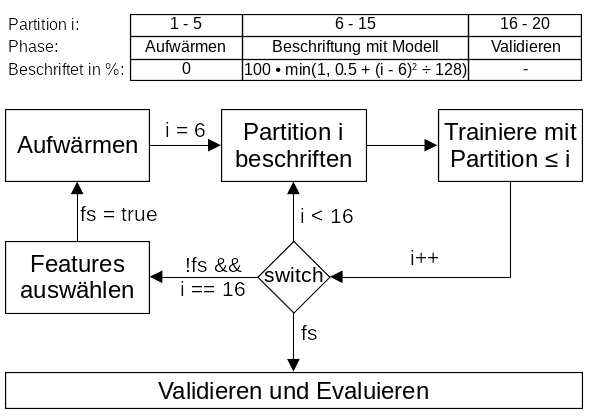
\includegraphics[width=\linewidth]{model/training_explained.png}
    \end{figure}
\end{frame}

% Entscheidungswälder besser als FFNN
% Entscheidungswälder skalieren besser mit steigender Standortkomplexität
% Standortansatz A skaliert besser als C
% $\leq8$ Entscheidungsbäume ausreichend
% Kleines Datenfenster ausreichend
\begin{frame}{Klassifizierungsgenauigkeit über Standortkomplexitäten}
    \begin{figure}
        \centering
        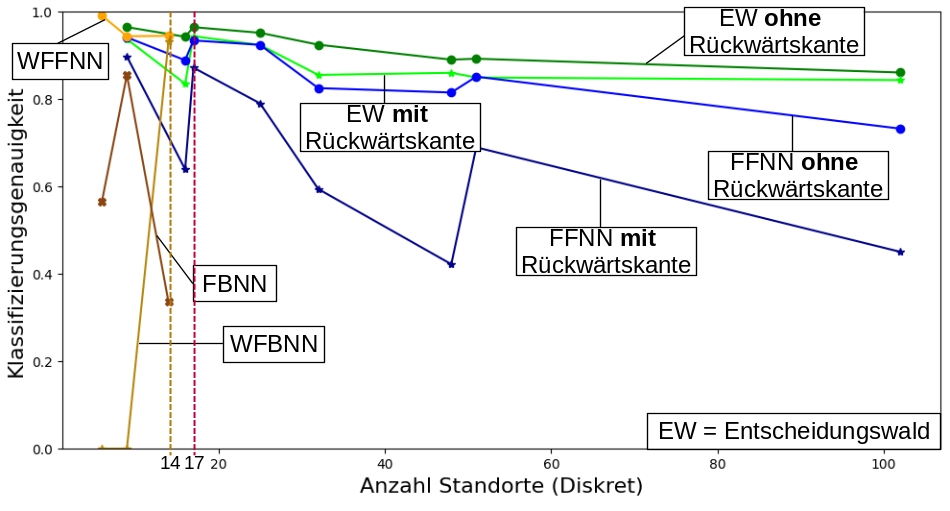
\includegraphics[width=\linewidth]{location_recognition/graph_comb.jpg}
    \end{figure}
\end{frame}

\begin{frame}{Wichtigkeit von Features}
    \begin{minipage}{.5\textwidth}
        \begin{enumerate}
            \item Basierend auf Entscheidungsregeln und Trainingsdaten
            \item Modifizieren der Testmenge und Fehler zur Originalmenge messen, z.~B. Permutationswichtigkeit oder Nullung
        \end{enumerate}
    \end{minipage}%
    \begin{minipage}{.5\textwidth}
        \centering
        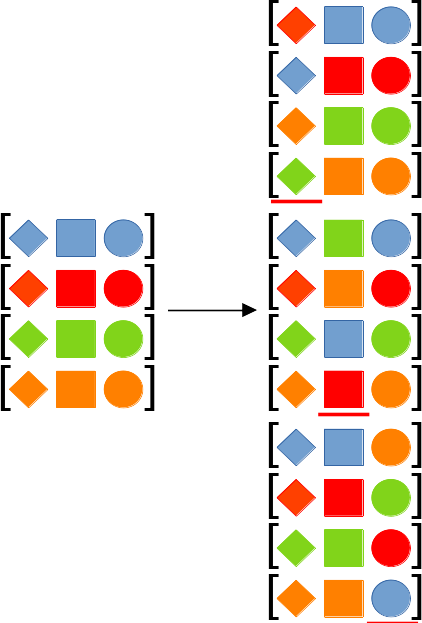
\includegraphics[width=0.9\linewidth]{model/permutatation_importance.png}
    \end{minipage}
\end{frame}

\begin{frame}{Permutationswichtigkeit - ML-Modelle mit Rückwärtskante}
    \begin{figure}
        \centering
        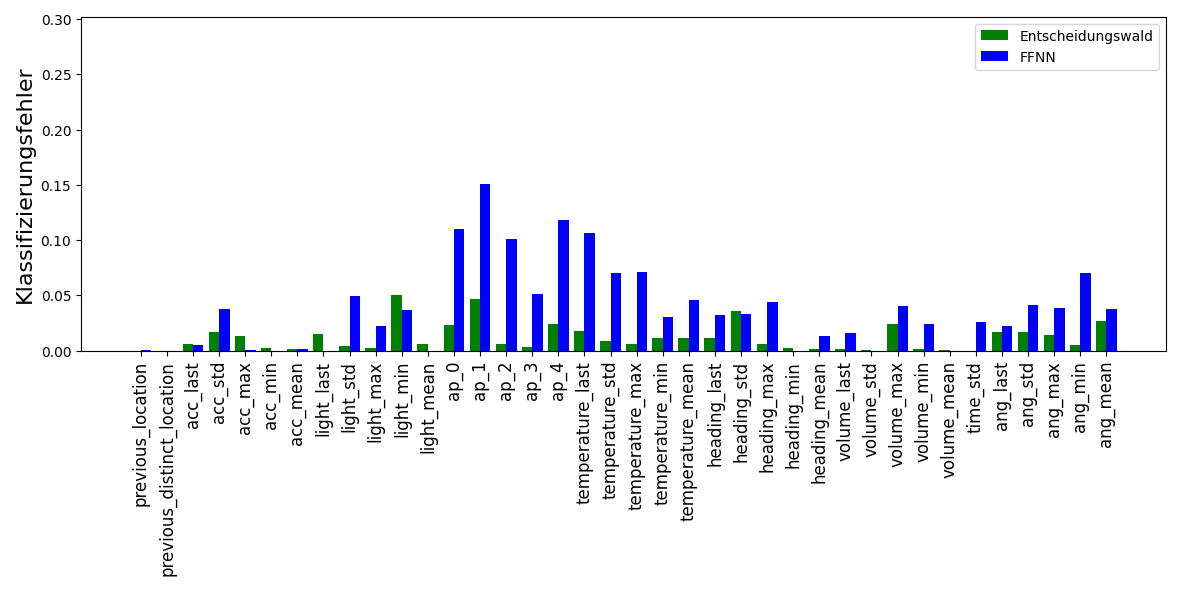
\includegraphics[width=\linewidth]{location_recognition/fi_consolidated.png}
    \end{figure}
\end{frame}

\begin{frame}{Permutationswichtigkeit - ML-Modelle ohne Rückwärtskante}
    \begin{figure}
        \centering
        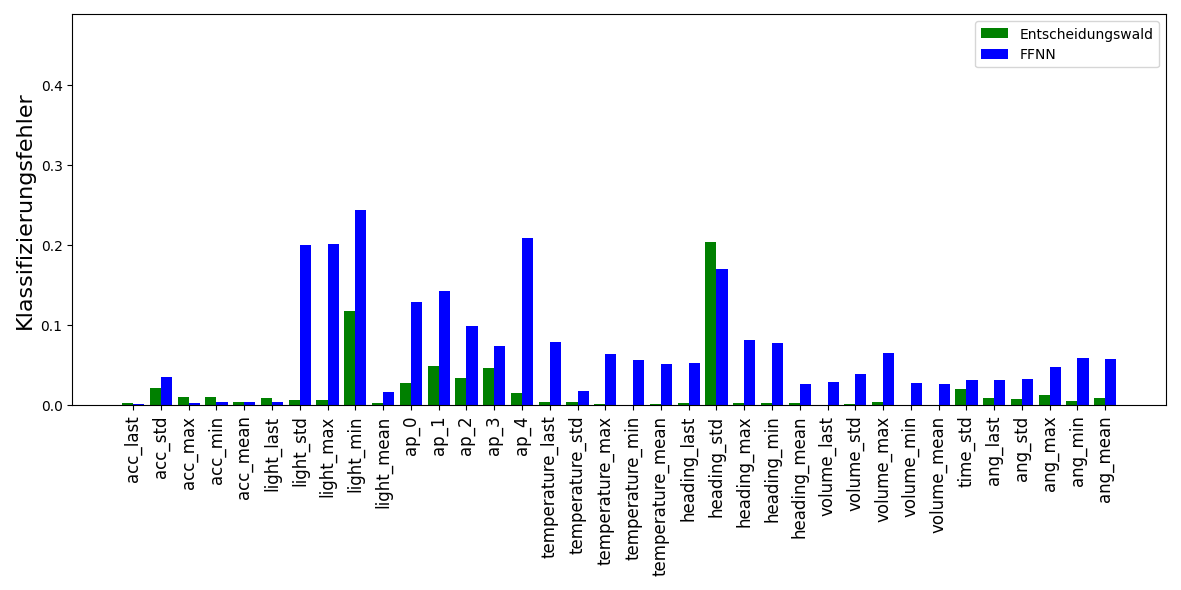
\includegraphics[width=\linewidth]{location_recognition/fi_consolidated_wo_fb.png}
    \end{figure}
\end{frame}

% Nullung der Sensorwerte indiziert Signifikanz
% Trainiert mit Fehlerdaten
% Entscheidungswälder und FFNN sehr stabil
% Sag wie viele Klassifizierungen nötig sind, damit der richtige Standort wieder gefunden wird
\begin{frame}{Fehlertoleranz}
    \footnotesize
    \begin{table}
        \setlength{\tabcolsep}{0.4em}
        \hspace*{-0.4cm}
        \begin{tabular}{ | l | c | c | c | c | }
            \hline
            Testmenge & Entscheidungswald & FFNN & Entscheidungswald & FNNN \\\hline
            & \multicolumn{2}{ c }{mit Rückwärtskante} & \multicolumn{2}{| c |}{ohne Rückwärtskante} \\\hline
            Licht & 4.46\%-Pkt. & 4.65\%-Pkt. & 5.28\%-Pkt. & 6.93\%-Pkt \\\hline
            Geräusch & 3.20\%-Pkt. & 5.00\%-Pkt. & 1.63\%-Pkt. & 5.11\%-Pkt. \\\hline
            Temperatur & 15.15\%-Pkt. & 6.60\%-Pkt. & 8.10\%-Pkt. & 13.50\%-Pkt. \\\hline
            Ausrichtung zum Magnetfeld & 3.32\%-Pkt. & 19.94\%-Pkt. & 2.51\%-Pkt. & 2.78\%-Pkt. \\\hline
            WLAN-Zugangspunkte & 2.60\%-Pkt. & 22.65\%-Pkt. & 3.74\%-Pkt. & 14.13\%-Pkt. \\\hline
            Accelerometer & 1.41\%-Pkt. & 9.52\%-Pkt. & 0.62\%-Pkt. & 1.33\%-Pkt. \\\hline
            Gyroskop & 8.52\%-Pkt. & 4.58\%-Pkt. & 0.91\%-Pkt. & 3.30\%-Pkt. \\\hline
            Permutierte Testmenge & 2.27\%-Pkt. & -0.13\%-Pkt. & 0.47\%-Pkt. & 0.93\%-Pkt. \\\hline
            \textbf{Durchschnitt} & \textbf{5,8\%-Pkt.} & \textbf{9,1\%-Pkt.} & \textbf{2,91\%-Pkt.} & \textbf{6,00\%-Pkt.} \\\hline
        \end{tabular}
    \end{table}
\end{frame}

\begin{frame}{Ressourcennutzung}
    \begin{itemize}
        \item Entscheidungswälder benötigen deutlich mehr Programmspeicher
        \item Entscheidungswälder benötigen deutlich weniger RAM
        \item Entscheidungswälder sind deutlich effizienter
        \item Programmgröße skaliert mit Standortkomplexität
        \item FFNNs zwischen 54\% und 97,6\% kleiner als Mians FFNNs (70KB bis 3KB)
        \item Enscheidungswälder bis zu 720\% größer als Mians FFNNs (ca. 1MB)
    \end{itemize}
\end{frame}

\section{Anomalieerkennung}
\begin{frame}{Anomalieerkennung}
    \begin{itemize}
        \item Anomalie := Klassifizierung: Momentaner Standort wurde nicht trainiert
        \item Unendliche viele mögliche Anomalien
        \item Training basierend auf Sensordaten nicht sinnvoll
        \item Klassifizierung ungewöhnlichen Verhaltes des Standortbestimmungsmodells
    \end{itemize}
\end{frame}

\begin{frame}{Summierte Klassifizierungsgenauigkeit in Datenfenster}
    \begin{figure}
        \centering
        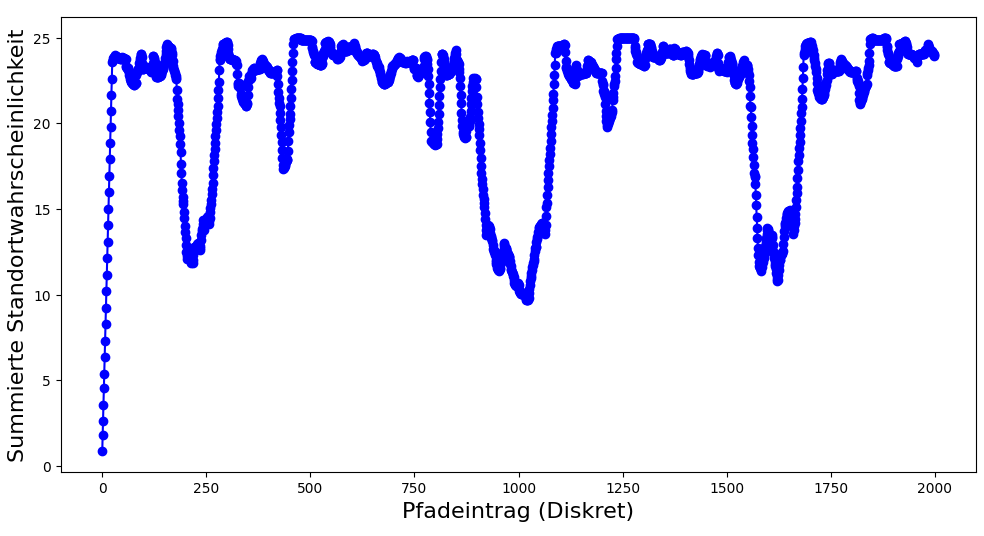
\includegraphics[width=\linewidth]{anomaly_detection/window_conf.png}
    \end{figure}
\end{frame}

\begin{frame}{Anzahl Standortänderungen in Datenfenster}
    \begin{figure}
        \centering
        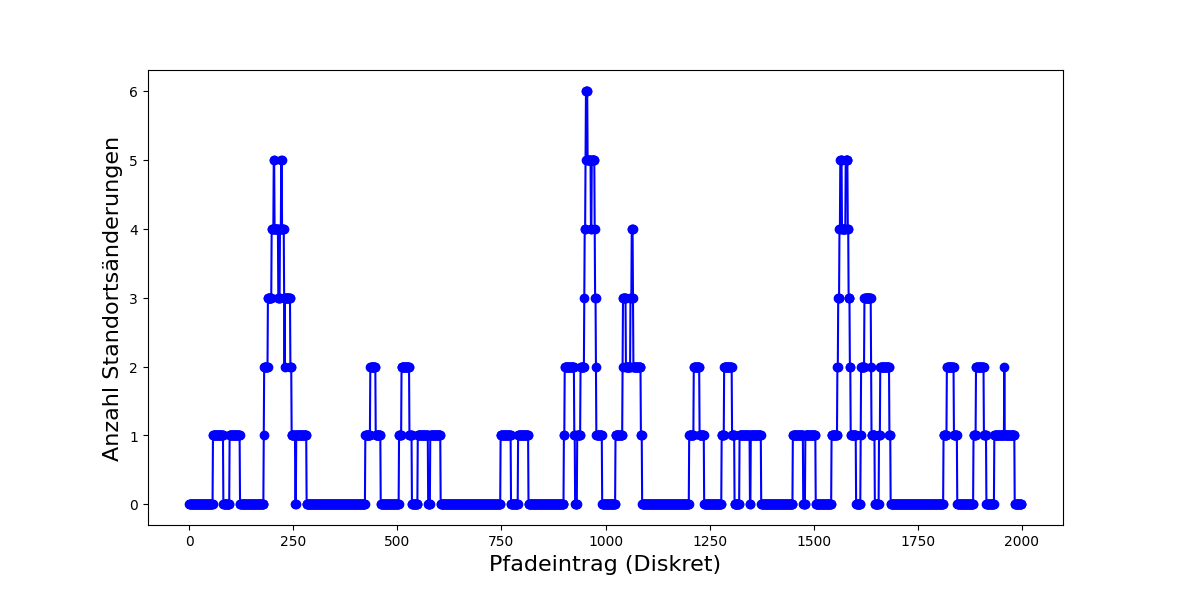
\includegraphics[width=\linewidth]{anomaly_detection/location_changes.png}
    \end{figure}
\end{frame}

\begin{frame}{Permutationswichtigkeit}
    \begin{figure}
        \centering
        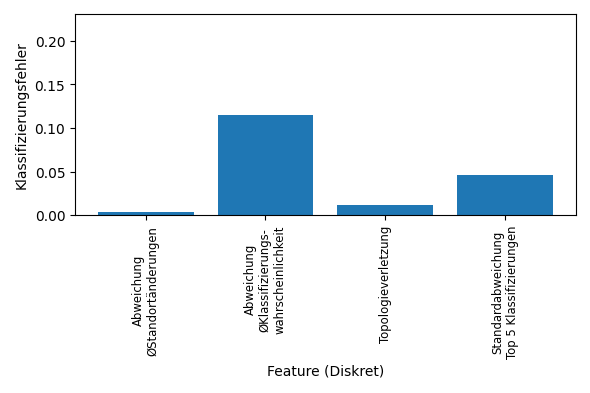
\includegraphics[width=\linewidth]{anomaly_detection/fi_anomaly_dt.png}
    \end{figure}
\end{frame}

\begin{frame}{Klassifizierungsergebnisse}
    \begin{minipage}{.5\textwidth}
        \begin{itemize}
            \item FFNN konnte \textbf{nicht} erfolgreich trainiert werden
            \item Entscheidungswald kann 52,52\% der Anomalien erkennen
            \item 2,95\% Falsch-Positiv Rate
            \item Klassifizierungsgenauigkeit abhängig von Erkennungsrate von ML-Modell und Standortkomplexität
        \end{itemize}
    \end{minipage}%
    \begin{minipage}{.5\textwidth}
        \centering
        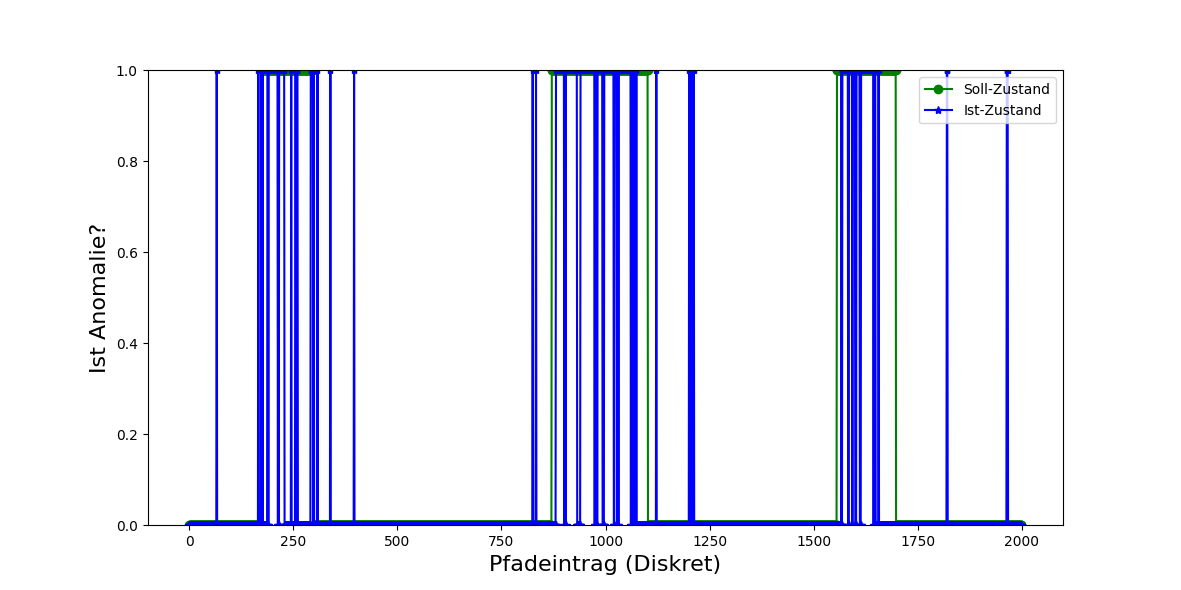
\includegraphics[width=\linewidth]{anomaly_detection/soll_vs_ist_anomaly.png} 
    \end{minipage}
\end{frame}

\section{Schlussfolgerungen}
\begin{frame}{Erkenntnisse dieser Arbeit}
    \begin{itemize}
        \item Entscheidungswälder skalieren besser als FFNN
        \item ML-Modelle ohne Rückwärtskante besser als mit
        \item 98,62\% bei 9 Standorten, 87,35\% bei 102 Standorten
        \item Anomalieerkennung: Bis zu 52,52\% bei Fehlerrate von 2,95\%
        \item Kleine Datenfenster sind ausreichend
        \item Geringere Ausführungszeit und klein genug
        \item Orte zu bestimmen ist besser als Orte und Pfade zu bestimmen
        \item Feature-Wichtigkeit abhängig vom Einsatzszenario
    \end{itemize}
\end{frame}

\begin{frame}[standout]
  Fragen?
\end{frame}

\begin{frame}{Wichtigkeit von Features - \texttt{feature\_importances\_}}
    \begin{figure}
        \centering
        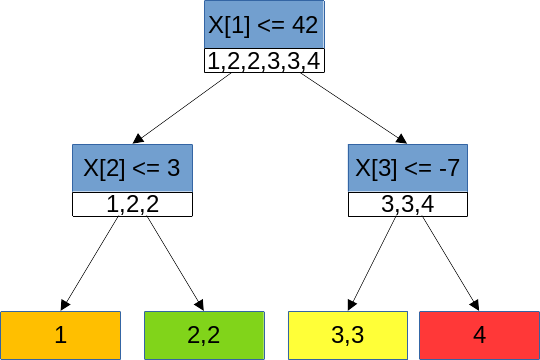
\includegraphics[width=\linewidth]{model/feature_importances.png}
    \end{figure}
\end{frame}

\begin{frame}{Simulationskarte von „Simple Square“}
    \begin{figure}
        \centering
        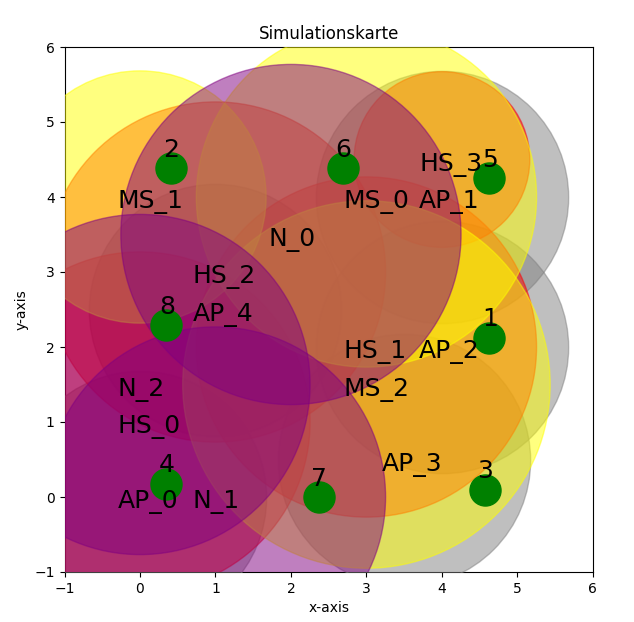
\includegraphics[width=0.75\linewidth]{settings/simple_square_simulation_map.png}
    \end{figure}
\end{frame}

\begin{frame}{Trainingsdaten pro Zyklus}
    \begin{figure}
        \centering
        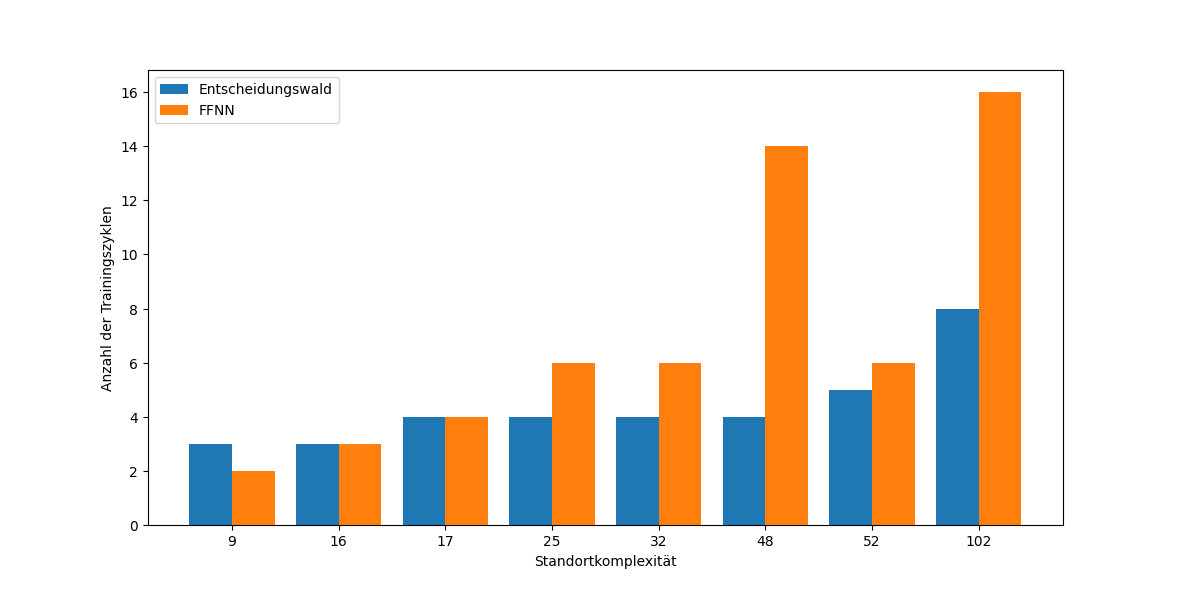
\includegraphics[width=\linewidth]{location_recognition/required_training_data.png}
    \end{figure}
\end{frame}

\begin{frame}{Anomalieerkennung: Klassifizierungsergebnisse}
    \footnotesize
    \begin{table}
        \setlength{\tabcolsep}{0.4em}
        \hspace*{-0.3cm}
        \begin{tabular}{ | p{1.5cm} | c | c | c | c | c | c | c | c | }
            \hline
            Standorte & 9 & 16 & 17 & 25 & 32 & 48 & 52 & 102 \\\hline
            \multicolumn{9}{ | l |}{$P(A)$}\\\hline
            DT & 82,59\% & 81,19\% & 87,14\% & 84,91\% & 79,06\% & 83,47\% & 81,93\% & 76,00\% \\\hline
            FFNN & 77,88\% & 77,88\% & 77,88\% & 77,88\% & 77,88\% & 77,88\% & 77,88\% & 77,88\% \\\hline
            Top. (DT) & 84,77\% & 30,57\% & 83,51\% & 79,76\% & 28,63\% & 24,97\% & 80,55\% & 29,47\% \\\hline
            Top. (KNN) & 86,10\% & 52,17\% & 77,72\% & 79,30\% & 45,06\% & 41,92\% & 74,77\% & 43,55\% \\\hline
            \multicolumn{9}{ | l |}{Anteil korrekt klassifiziert, indem Anomalie vorlag}\\\hline
            DT & 34,86\% & 35,52\% & 52,58\% & 50,92\% & 32,21\% & 50,64\% & 23,21\% & 1,92\% \\\hline
            FFNN & 0,00\% & 0,00\% & 0,00\% & 0,00\% & 0,00\% & 0,00\% & 0,00\% & 0,00\% \\\hline
            \multicolumn{9}{ | l |}{Anteil korrekt klassifiziert, indem keine Anomalie vorlag}\\\hline
            DT & 96,14\% & 94,41\% & 97,05\% & 95,83\% & 92,48\% & 93,13\% & 98,96\% & 97,18\% \\\hline
            FFNN & 100,00\% & 100,00\% & 100,00\% & 100,00\% & 100,00\% & 100,00\% & 100,00\% & 100,00\% \\\hline
        \end{tabular}
    \end{table}
\end{frame}

\begin{frame}{$P(B\leq5)_{\text{cont}}$ - Auswirkung von maximaler Baumhöhe}
    \begin{figure}
        \centering
        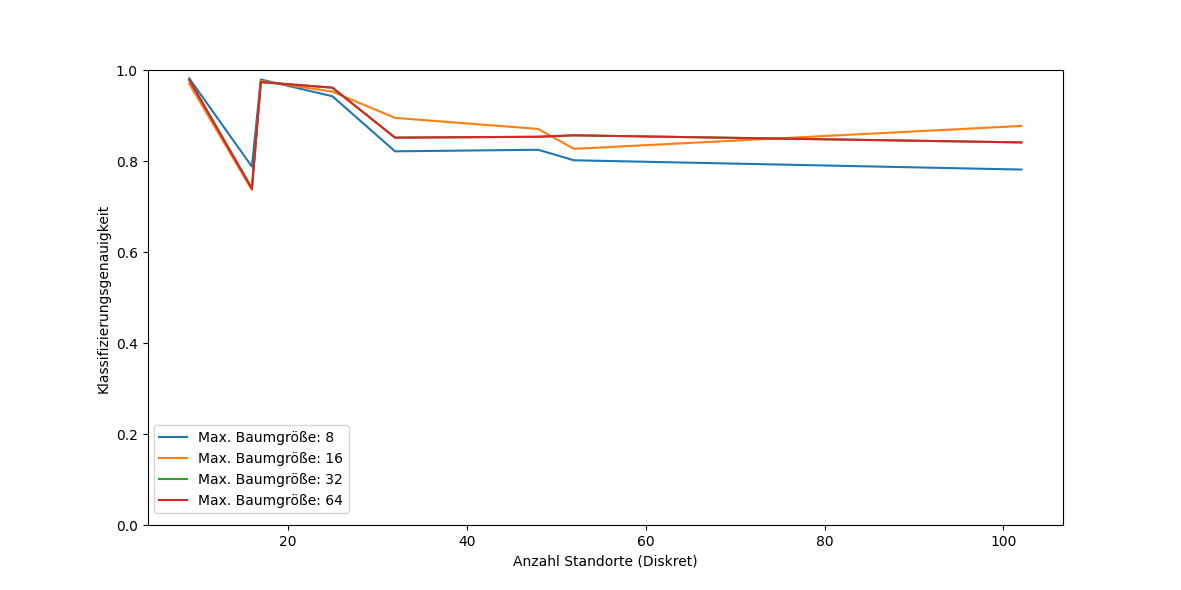
\includegraphics[width=\linewidth]{location_recognition/multiple_best_by_group_dt_max_depth_acc_5_cont.png}
    \end{figure}
\end{frame}

\begin{frame}{$P(B\leq5)_{\text{cont}}$ - Auswirkung von Waldgröße}
    \begin{figure}
        \centering
        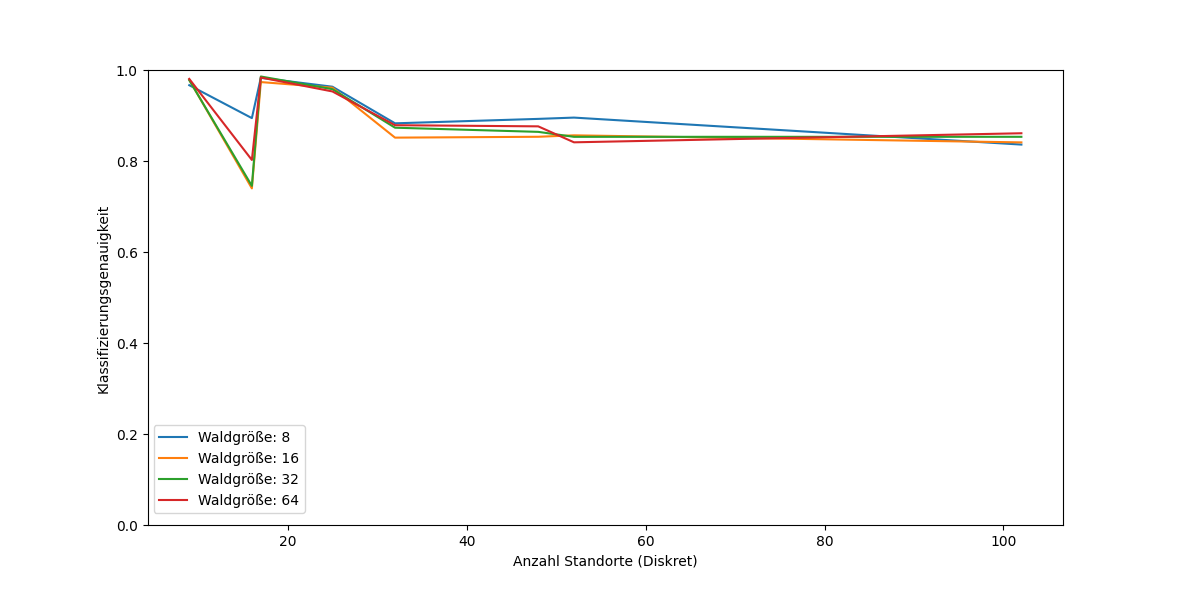
\includegraphics[width=\linewidth]{location_recognition/multiple_best_by_group_dt_trees_acc_5_cont.png}
    \end{figure}
\end{frame}

\begin{frame}{$P(B\leq5)_{\text{cont}}$ - Auswirkung von Anzahl Neuronen}
    \begin{figure}
        \centering
        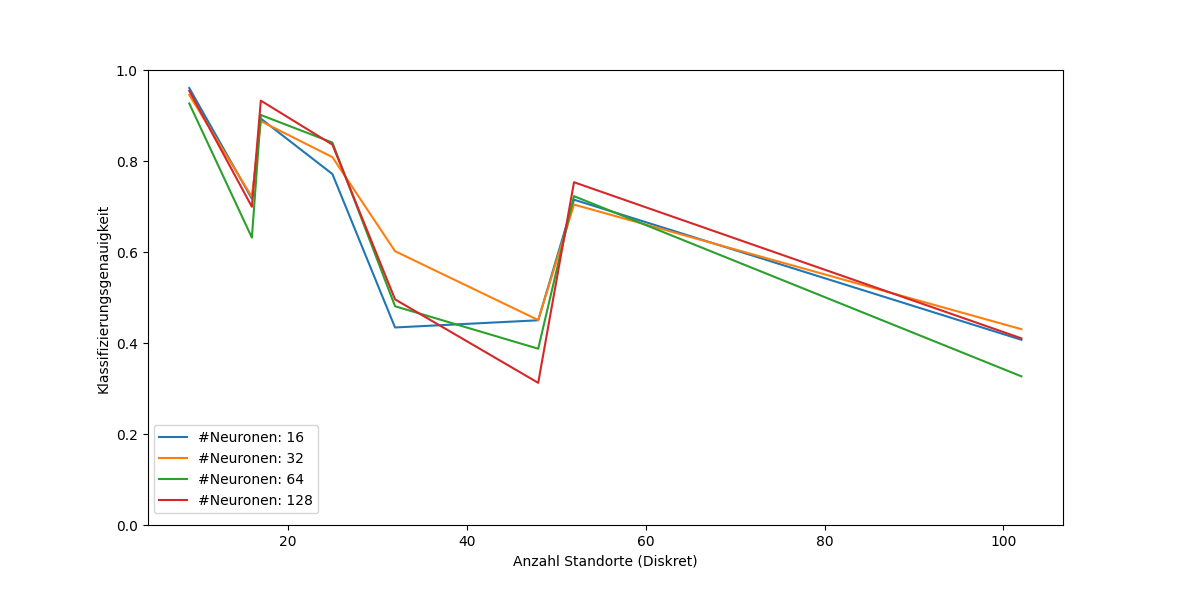
\includegraphics[width=\linewidth]{location_recognition/multiple_best_by_group_knn_neurons_acc_5_cont.png}
    \end{figure}
\end{frame}

\begin{frame}{$P(B\leq5)_{\text{cont}}$ - Auswirkung von Anzahl verdeckte Schichten}
    \begin{figure}
        \centering
        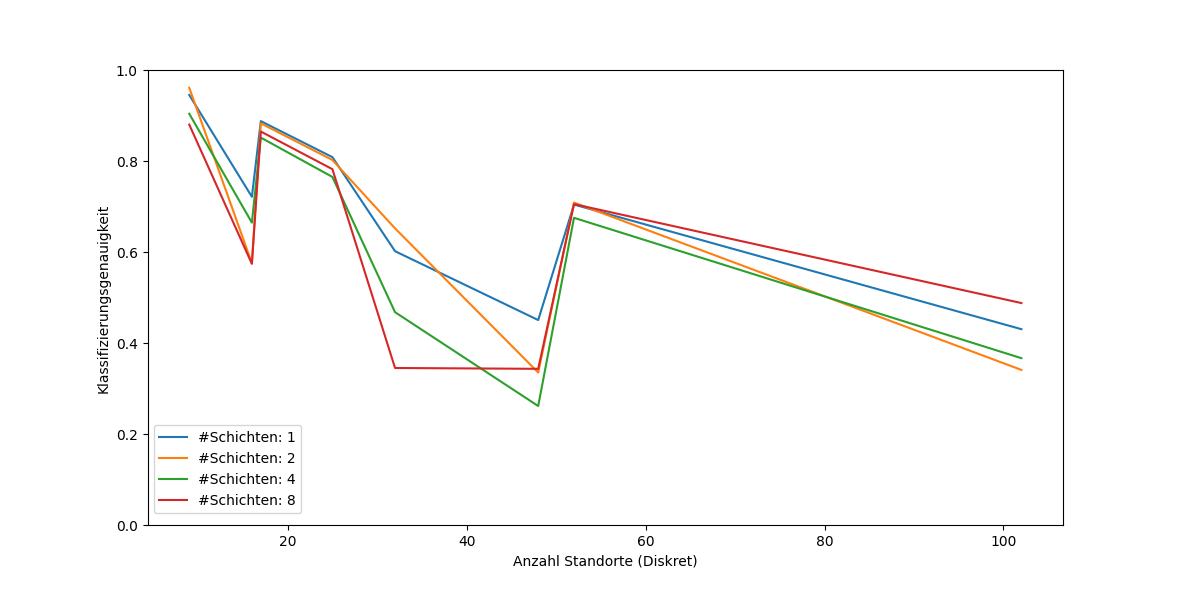
\includegraphics[width=\linewidth]{location_recognition/multiple_best_by_group_knn_layers_acc_5_cont.png}
    \end{figure}
\end{frame}

\begin{frame}{Route: "Many Corners"}
    \begin{figure}
        \centering
        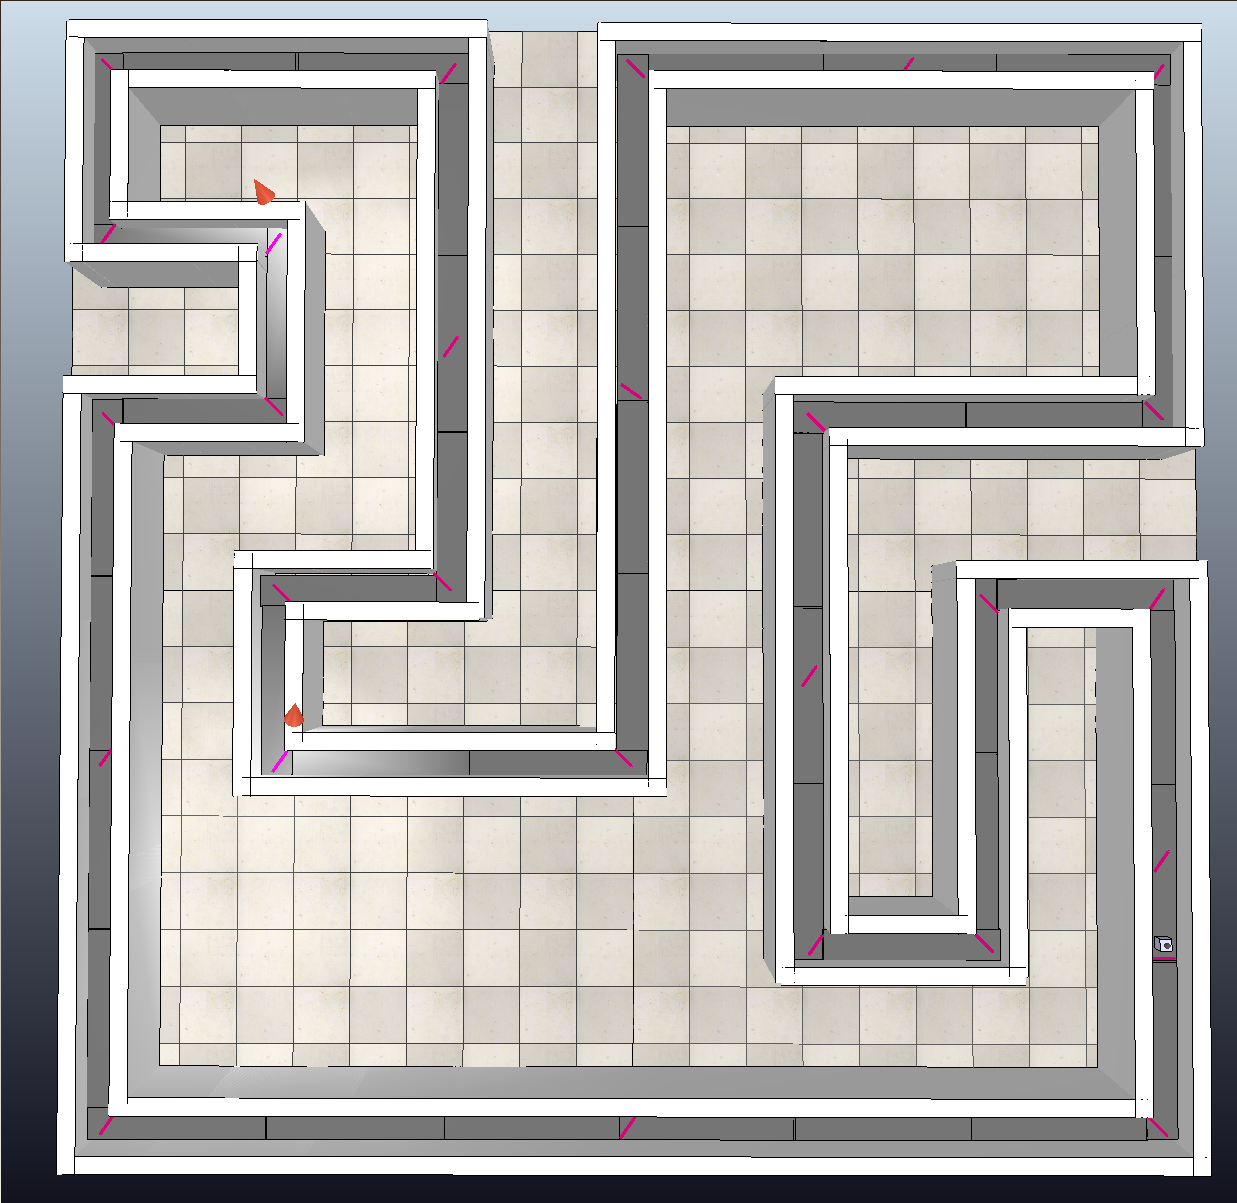
\includegraphics[width=0.8\linewidth]{routes/many_corners.png}
    \end{figure}
\end{frame}

\begin{frame}{Route: "Simple Square"}
    \begin{figure}
        \centering
        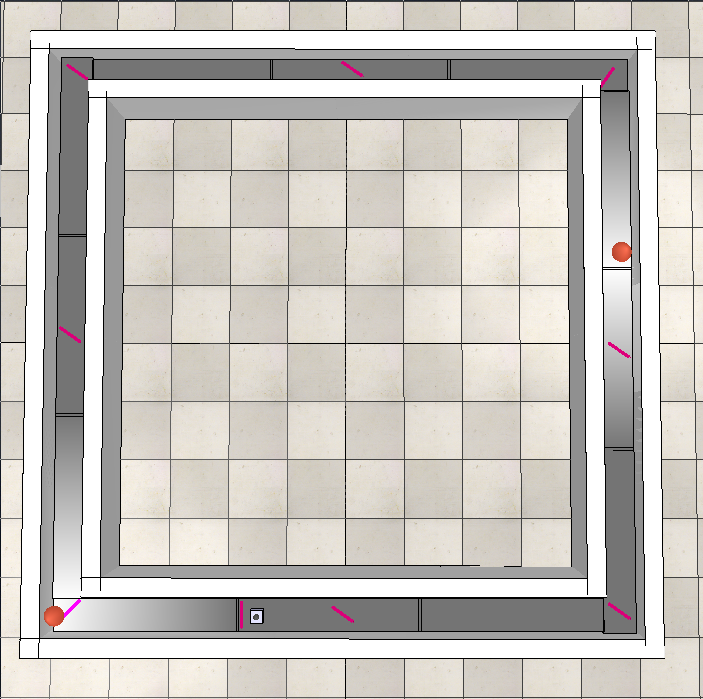
\includegraphics[width=0.8\linewidth]{routes/simple_square.png}
    \end{figure}
\end{frame}

\begin{frame}{Route: "Long Rectangle"}
    \begin{figure}
        \centering
        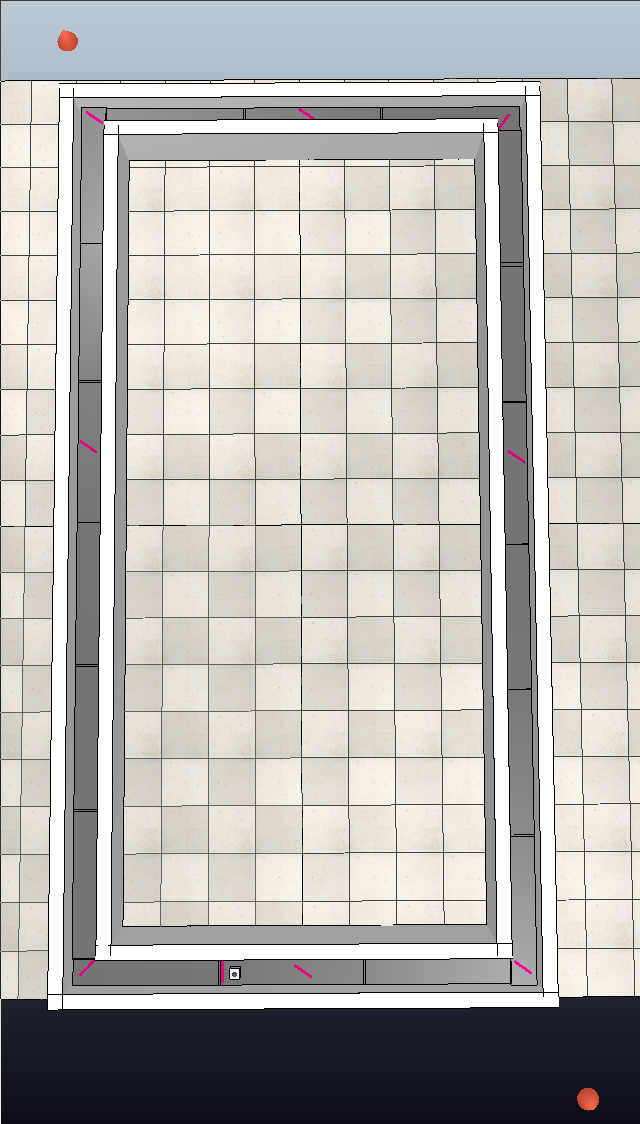
\includegraphics[angle=90,width=\linewidth]{routes/long_rectangle.png}
    \end{figure}
\end{frame}

\begin{frame}{Route: "Rectangle with Ramp"}
    \begin{figure}
        \centering
        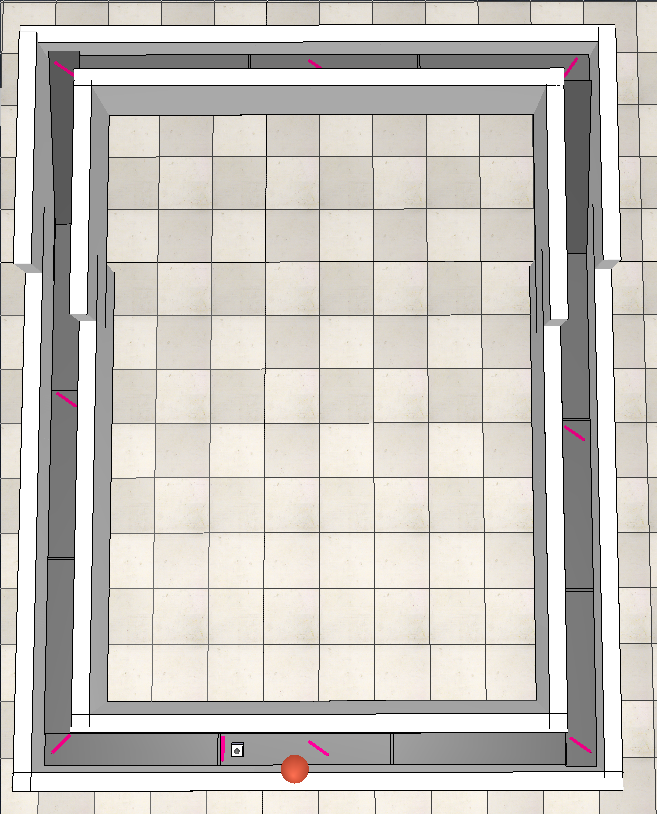
\includegraphics[angle=90,width=0.9\linewidth]{routes/rectangle_with_ramp.png}
    \end{figure}
\end{frame}

\end{document}

